\documentclass[landscape]{article}
\usepackage[pdftex]{graphicx,color,hyperref}
\pagestyle{empty}
\oddsidemargin  -0.5 in
\evensidemargin -0.5 in
\headheight     0 in
\topmargin      -1 in
\textheight     7.7 in
\textwidth      10 in
\newenvironment{slide}{\mbox{ }\vfill}{\vfill \mbox{ } \pagebreak}
\newenvironment{lastslide}{\mbox{ }\vfill}{\vfill \mbox{ }}
\begin{document}
\huge
\renewcommand{\labelitemi}{-}
\setlength{\parindent}{0 cm}

\begin{slide}
  \vfill
  \begin{center}
    {\Huge Calculating hadronic cross-section}

    \vspace{0.5 cm}
    {\Huge for runs at the same energy}

    \vspace{0.5 cm}
    {\Huge and getting the same answer}

    \vfill Jim Pivarski
  \end{center}
  \vfill
\end{slide}

\begin{slide}
  Previously, I measured hadronic efficiency to high precision

  \vfill
  Luminosity measurement in two parts:
  \begin{enumerate}
    \item Calculated luminosity is correct for each run relative to all
    others (remember, I'm doing scans)

    \item Absolute magnitude of luminosity is correct
  \end{enumerate}

  \vfill
  Today, I focus on \#1

  \vfill
  Contents:
  \begin{itemize}
    \item Gamgam cuts for luminosity

    \item Trigger efficiency for gamgams

    \item Look at hadronic cross-section of $\Upsilon(3S)$ continuum:
    see fluctuations

    \item Why?  Sensitivity to CC calibration

    \item Change gamgam {\it and} hadron cuts to reduce sensitivity

    \item Will this be a problem for my hadronic efficiency measurement?  No.
  \end{itemize}
\end{slide}

\begin{slide}
  $e^+e^- \to \gamma\gamma$ (gamgam)

  \vspace{0.5 cm}
  (Why use gamgam?  $e^+e^-$ and $\mu^+\mu^-$ interfere with $\Upsilon$ across resonance)

  \vfill
  \begin{tabular}{p{0.7\linewidth} p{0.3\linewidth}}
    \begin{minipage}{\linewidth}
      Initial cuts:
      \begin{enumerate}
        \item BhabhaBarrel trigger line (the only neutral trigger in CLEO-III)

        \item Second-biggest shower (E2) $>$ 90\% eBeam

        \item Zero ``quality'' tracks

        \item $|\cot\theta_1 + \cot\theta_2|$ $<$ 0.1 (back-to-back in $\theta$)

        \item $|\sin(\phi_1 - \phi_2)|$ $<$ 0.04 (back-to-back in $\phi$, avoiding bhabhas)

        \item asymmetric cut on $\cot\theta$: upper limit of 1.28, 1.18 \\
	  ($= \cos\theta$ of 0.79 $=$ barrel)

        \item asymmetric cut on $\cot\theta$: lower limit of 0.05, 0.15 to
        avoid trigger inefficiency at the center of the detector
      \end{enumerate}
    \end{minipage} & \begin{minipage}{\linewidth}
      \vspace{3.5 cm}
      \begin{center} Asymmetric cut: \end{center}

      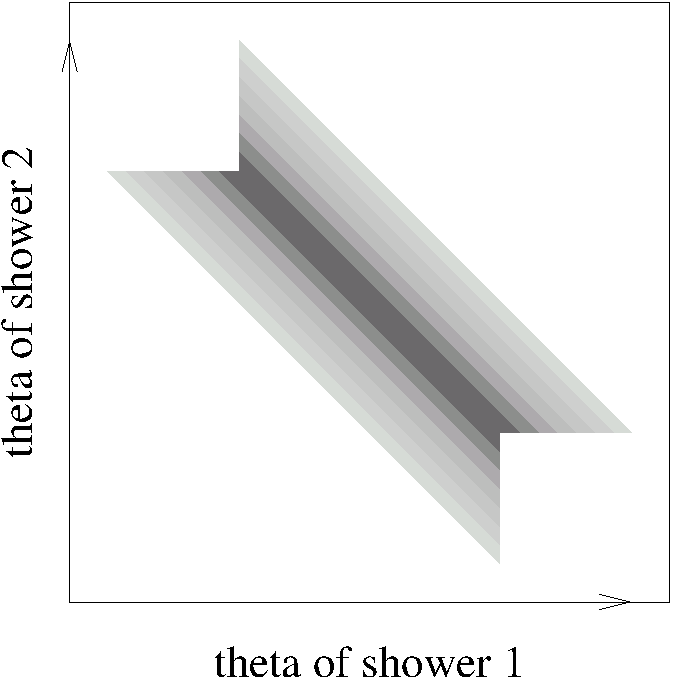
\includegraphics[width=\linewidth]{explain_asymmetric_cut.pdf}
    \end{minipage}
  \end{tabular}
\end{slide}

\begin{slide}
  \vfill BarrelBhabha trigger requires two CBHI clusters ($>$ 1.5 GeV
  each): on opposite sides of the detector (edge effect near
  $\cos\theta = 0$)

  \vfill Can be measured by identifying bhabhas with gamgam cuts and
  0.04 $<$ $|\sin(\phi_1 - \phi_2)|$ $<$ 0.25, and asking for
  BarrelBhabha trigger bit.  (Corrected for $\theta$ dependence.)

  \vfill \begin{center}
    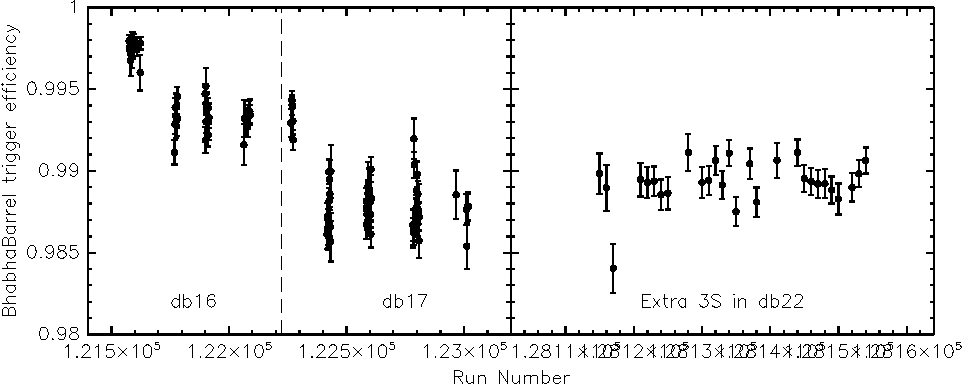
\includegraphics[width=\linewidth]{prepforpta2.pdf}
  \end{center}
\end{slide}

\begin{slide}
  Why does trigger efficiency have steps?

  \vfill Three tiles become very inefficient at different times during
  CLEO-III non-4S.

  \vfill They were all fixed before the end of CLEO-III.

  \vfill
  \begin{center}
    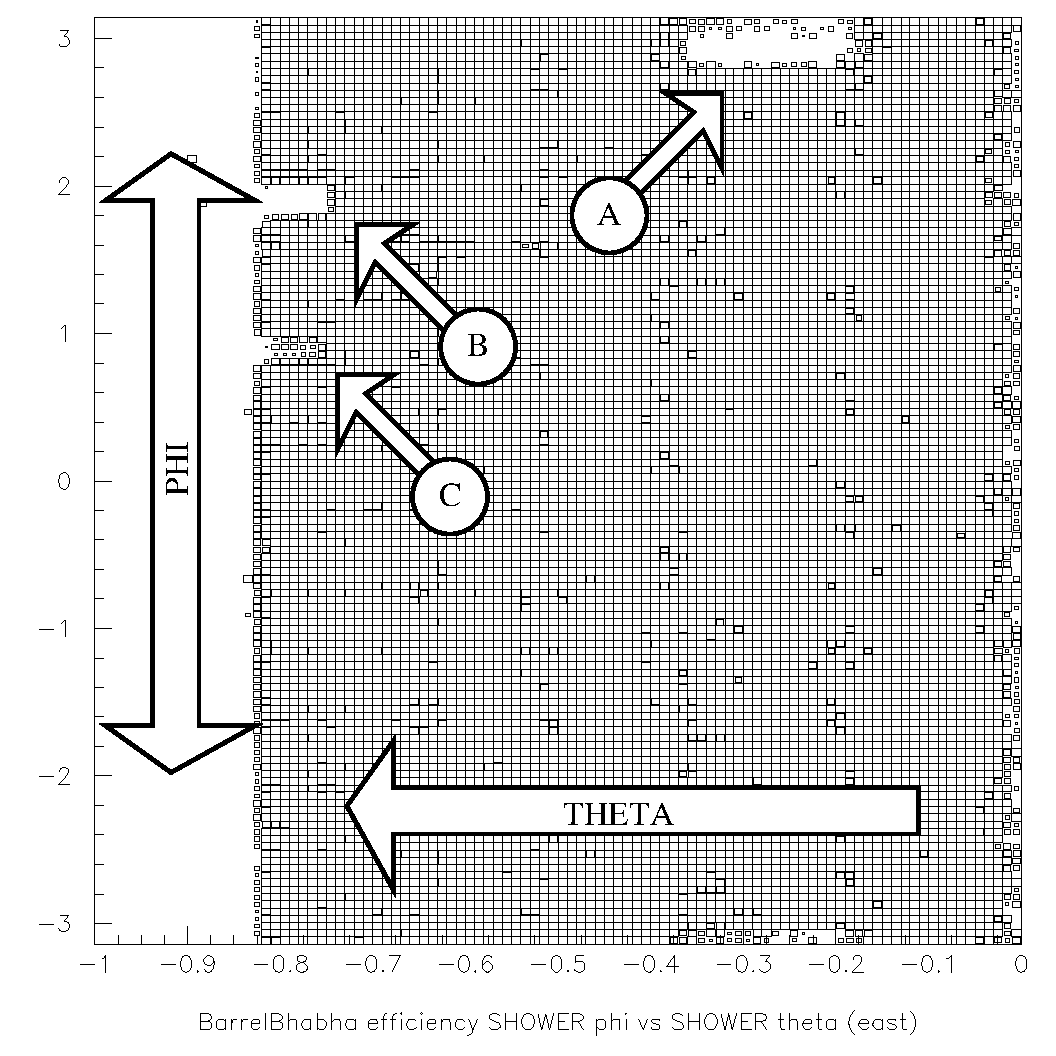
\includegraphics[width=0.45\linewidth]{plottrig_blocks2.pdf} \hfill
    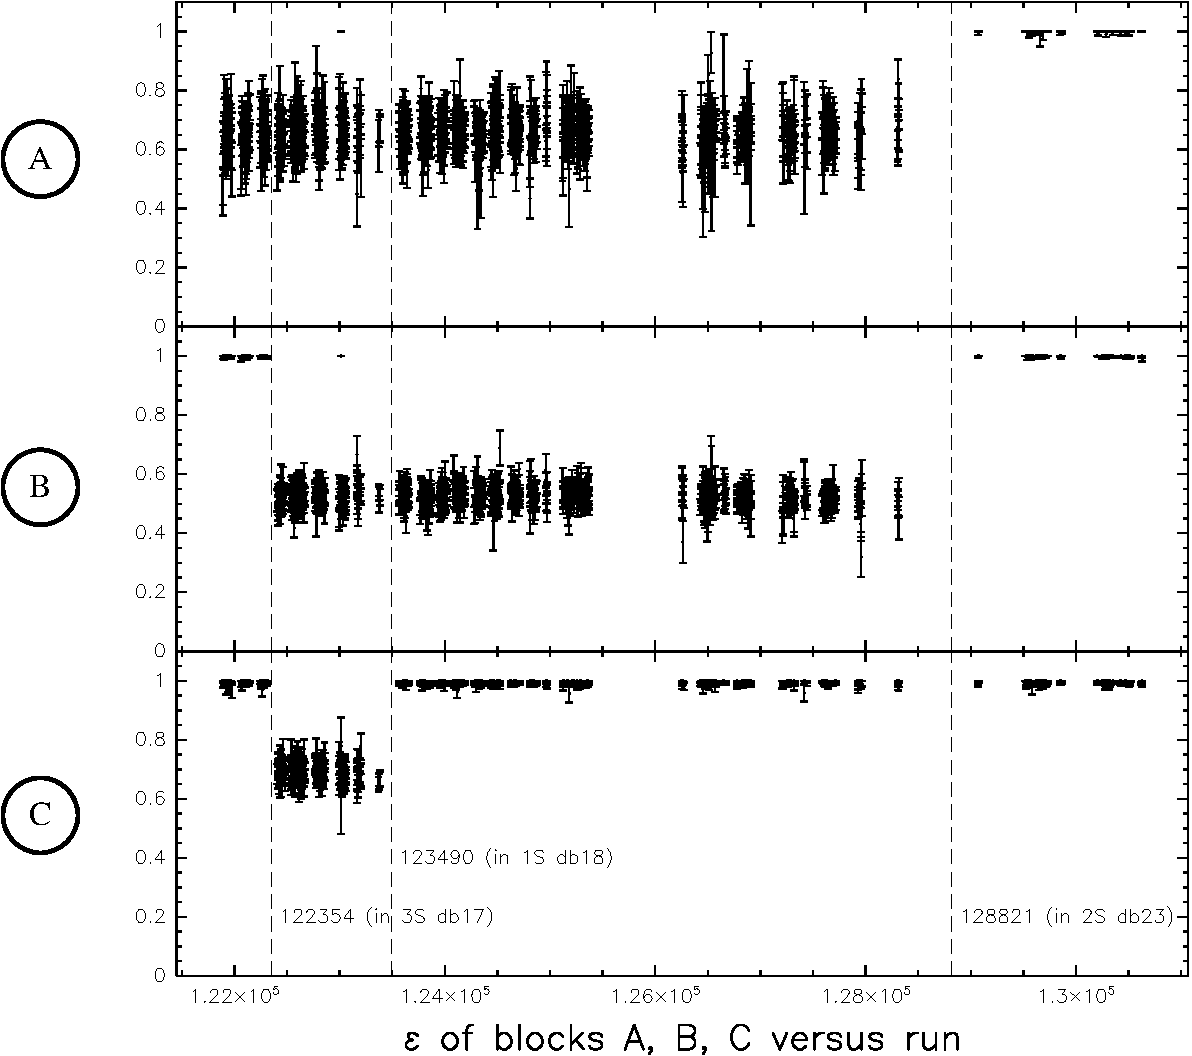
\includegraphics[width=0.45\linewidth]{plottrig_blocks_vrun2.pdf}
  \end{center}
\end{slide}

\begin{slide}
  So I additionally exclude these blocks from my gamgam cuts

  \vfill Trigger efficiency {\it given} other gamgam cuts is now
  99.8\%

  \vfill
  \begin{center}
    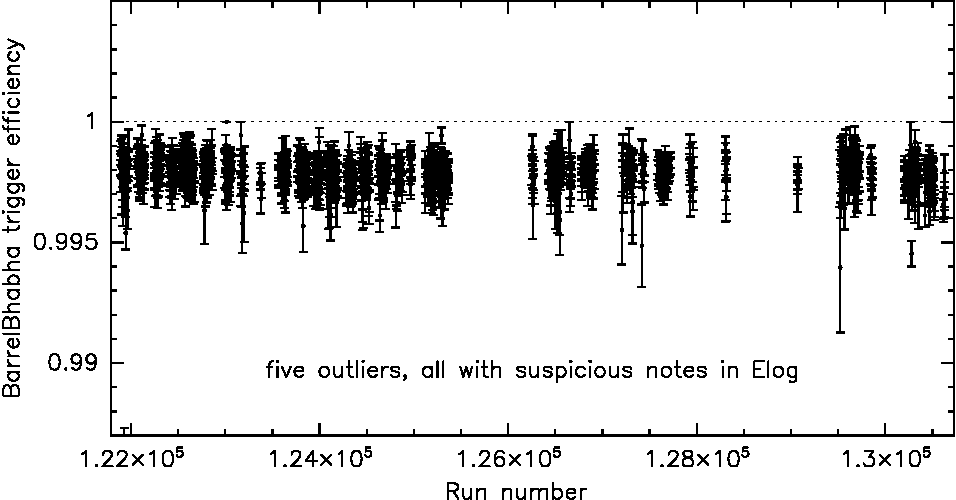
\includegraphics[width=\linewidth]{afterexclude.pdf}
  \end{center}
\end{slide}

\begin{slide}
  \begin{center}

    \vfill \begin{minipage}{0.85\linewidth} Test the hypothesis that
      run-by-run luminosity is stable by calculating hadronic
      cross-section for $\Upsilon(3S)$ continuum (9 running periods)
    \end{minipage}

    \vfill \begin{minipage}{0.85\linewidth}
      Caveats:
      \begin{itemize}
        \item Hadronic efficiency that I measured before doesn't apply to
          continuum--- but it should be constant with time

        \item Other luminosity systematics remain, but none of them depend
	  on time
      \end{itemize}
    \end{minipage}

    \vfill \begin{minipage}{0.85\linewidth}
      $\Longrightarrow$ This is hadronic cross-section $\times$
      unknown constant
    \end{minipage}

  \vfill
  \end{center}
\end{slide}

\begin{slide}
  \begin{center}
    \Huge Fluctuations!!!  \hspace{0.5 cm} $\chi^2/$ndf $=$ 25.7 / 8 \hspace{0.5 cm} $\Rightarrow$ 0.1\% C.L. \\

    \vfill 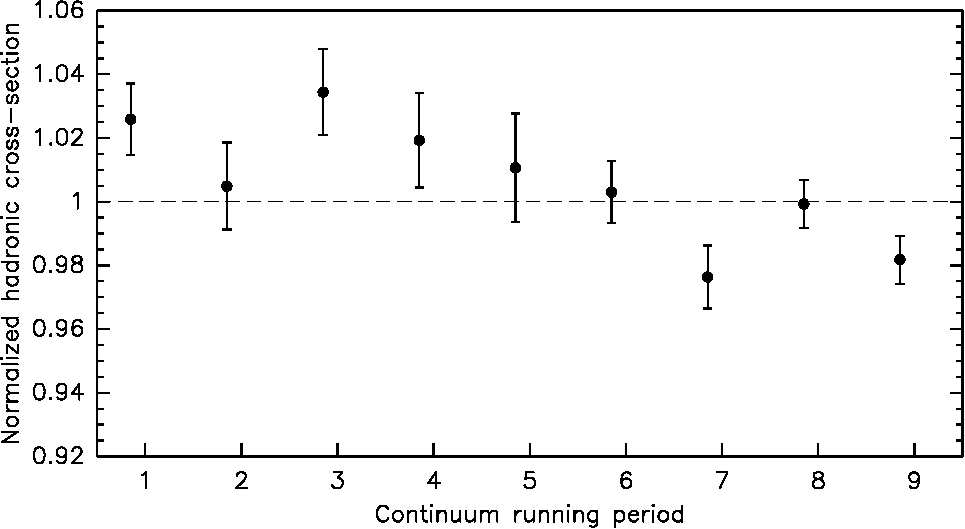
\includegraphics[width=\linewidth]{prepforpta4_0.pdf}
  \end{center}
\end{slide}

\begin{slide}
  Take a closer look at points 3 and 7 (the most extreme)

  \vfill Cuts most responsible for difference in hadronic
  cross-section: shower energy cuts

  \vfill CC calibration drifted 6 MeV between points 3 and 7

  \vfill
  \begin{center}
    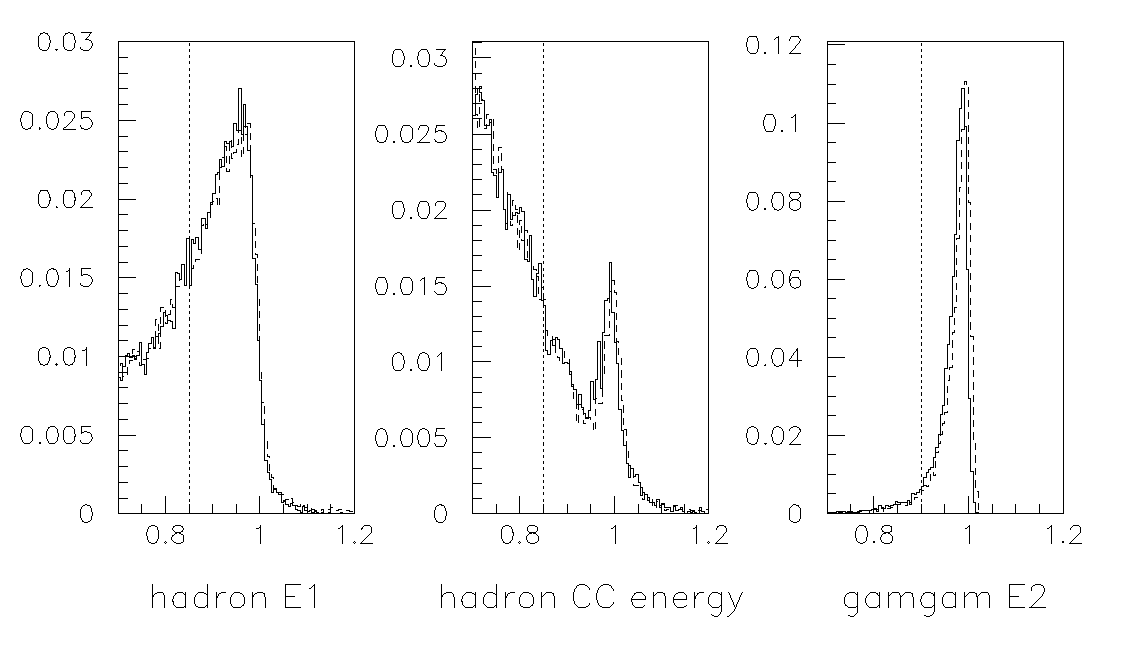
\includegraphics[width=0.9\linewidth]{forptatalk.pdf}
  \end{center}
\end{slide}

\begin{slide}
  \vfill
  \begin{center}
    \begin{minipage}{0.85\linewidth} Does this matter? \end{minipage}

    \vfill \begin{minipage}{0.85\linewidth} It is the continuum
      yield which is fluctuating--- if drift is slow, I can subtract only
      ``nearby'' continuum \end{minipage}

    \vfill \begin{minipage}{0.85\linewidth} But how close is close
      enough?  This problem limits how much on-resonance data I can use in
      an unknown way \end{minipage}

    \vfill \begin{minipage}{0.85\linewidth} Also, $\Upsilon(2S)$
    continuum is not all near on-resonance \end{minipage}
  \end{center}
  \vfill
\end{slide}

\begin{slide}
  \begin{center}
    \vfill
    \begin{minipage}{0.85\linewidth} Can my cuts be modified to make this safer?  {\Huge YES!} \end{minipage}

    \vfill \begin{minipage}{0.85\linewidth} anti-bhabha cuts in hadron \end{minipage}

    \vspace{1 cm} \begin{minipage}{0.85\linewidth} \begin{tabular}{p{0.75 cm} p{8 cm} p{3 cm} p{8 cm}}
	& \begin{minipage}{\linewidth}
	  \begin{center}
	    E1 $<$ 0.85 eBeam \\
	    P2 $<$ 0.85 eBeam \\
	    CC energy $<$ 0.85 eCOM \end{center} \end{minipage} &
	\begin{minipage}{\linewidth} $\longrightarrow$ \end{minipage} &
	\begin{minipage}{\linewidth} P1 $<$ 0.8 eBeam \end{minipage}
      \end{tabular} \end{minipage}

    \vfill \begin{minipage}{0.85\linewidth} energy cut in gamgam \end{minipage}

    \vspace{0.5 cm} \begin{minipage}{0.85\linewidth} \begin{tabular}{p{0.75 cm} p{8 cm} p{3 cm} p{8 cm}}
	& \begin{minipage}{\linewidth} \begin{center} E2 $>$ 0.9 eBeam \end{center} \end{minipage} &
	\begin{minipage}{\linewidth} $\longrightarrow$ \end{minipage} &
	\begin{minipage}{\linewidth} E2 $>$ 0.7 eBeam \end{minipage}
      \end{tabular} \end{minipage}

    \vfill \begin{minipage}{0.85\linewidth} (E1,2 are biggest shower energies, P1,2 are biggest track momenta) \end{minipage}
  \end{center}
  \vfill
\end{slide}

\begin{slide}
  \begin{center}
    \begin{tabular}{p{0.35\linewidth} l r}
      old hadron, gamgam at 0.9 & $\chi^2/$ndf $=$ 25.7 / 8 & $\Rightarrow$ 0.1\% C.L. \\
      old hadron, gamgam at 0.7 & $\chi^2/$ndf $=$ 20.9 / 8 & $\Rightarrow$ 0.7\% C.L. \\
      new hadron, gamgam at 0.7 & $\chi^2/$ndf $=$ 12.7 / 8 & $\Rightarrow$ 12\% C.L.
    \end{tabular}

    \vfill 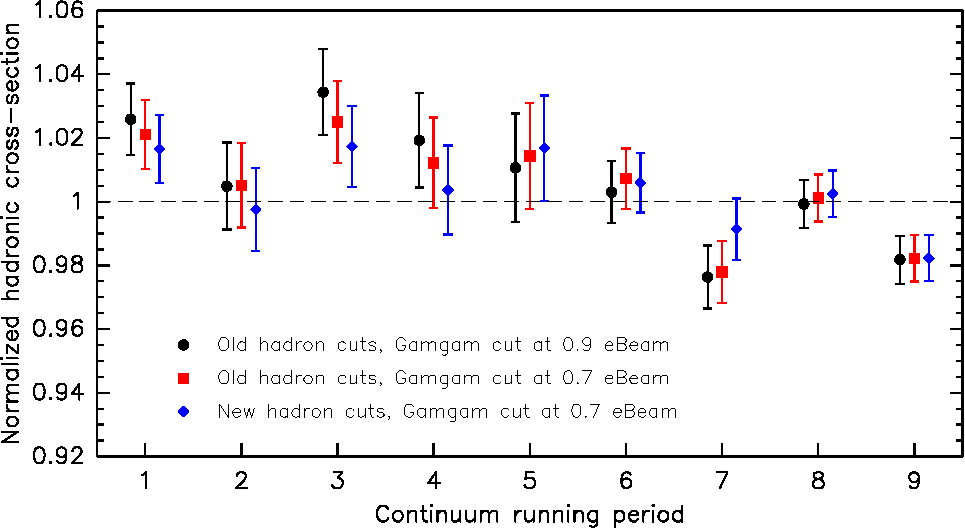
\includegraphics[width=\linewidth]{prepforpta4.pdf}
  \end{center}
\end{slide}

\begin{slide}
  \begin{center}
    \vfill
    Old hadron cuts, Gamgam cut at 0.9 eBeam

    \vfill
    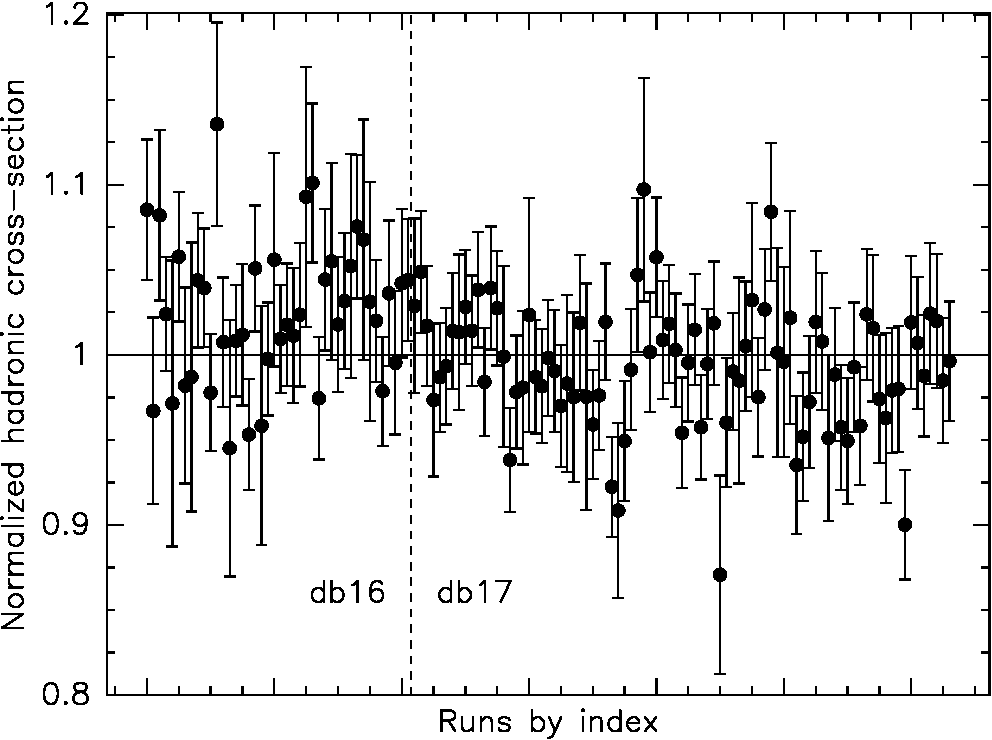
\includegraphics[width=0.85\linewidth]{prepforpta3_oldhadronalloldgam.pdf}
  \end{center}
\end{slide}

\begin{slide}
  \begin{center}
    \vfill
    Old hadron cuts, Gamgam cut at 0.7 eBeam

    \vfill
    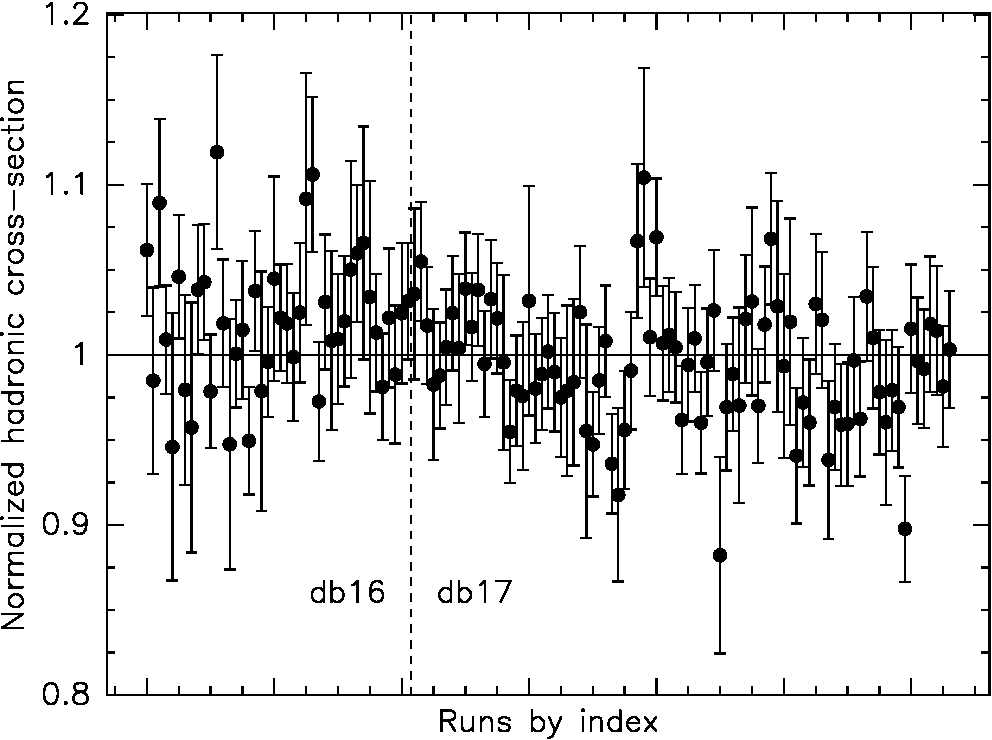
\includegraphics[width=0.85\linewidth]{prepforpta3_oldhadronall.pdf}
  \end{center}
\end{slide}

\begin{slide}
  \begin{center}
    \vfill
    New hadron cuts, Gamgam cut at 0.7 eBeam

    \vfill
    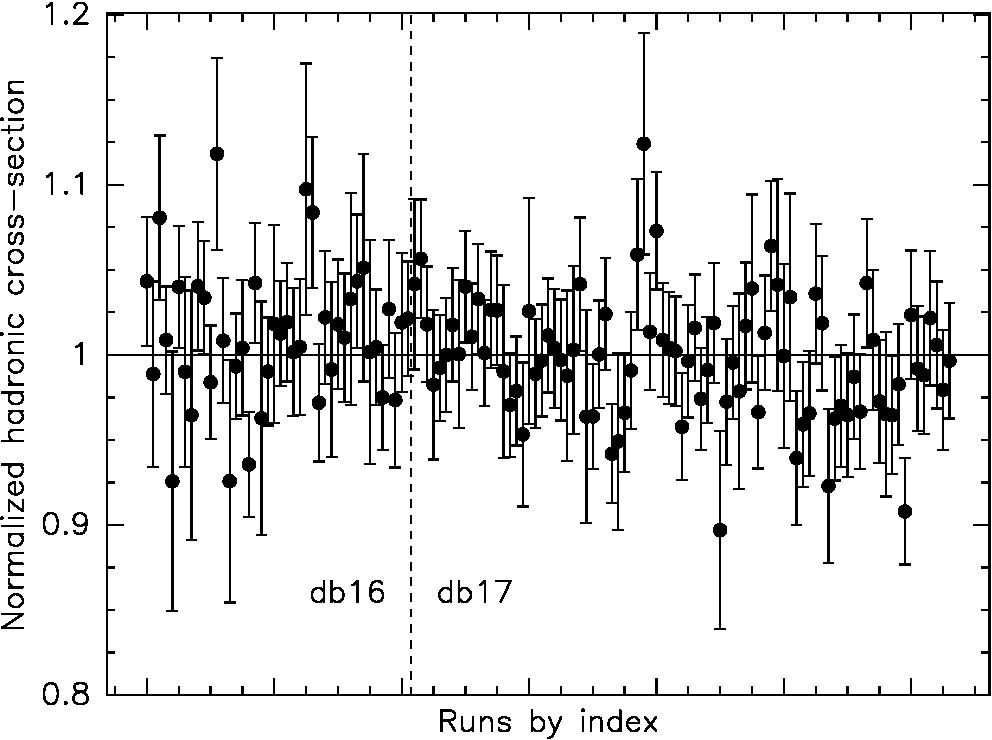
\includegraphics[width=0.85\linewidth]{prepforpta3.pdf}
  \end{center}
\end{slide}

\begin{slide}
  \vfill
  \begin{center}
    \begin{minipage}{0.85\linewidth} Are my new cuts as effective at cutting bhabha backgrounds? \end{minipage}

    \vfill \begin{minipage}{0.85\linewidth} Essentially. \end{minipage}

    \vspace{0.5 cm} \begin{minipage}{0.85\linewidth} \begin{center} \begin{tabular}{p{0.5\linewidth} p{0.1\linewidth} p{0.13\linewidth} p{0.13\linewidth}}
	& & old cuts & new cuts \\
	fraction of continuum subtraction which is bhabha subtraction$^*$ & & $\sim$ 7.3\% & $\sim$ 8.4\% \\
      \end{tabular} \end{center} \end{minipage}

    \vfill \begin{minipage}{0.85\linewidth} This means that changes to my draft CBX are minimal: I need to re-create plots and figures. \end{minipage}

    \vfill \mbox{\vspace{1 cm}} \begin{minipage}{0.85\linewidth}
    ($^*$How did I determine that?  $E_{\mbox{\normalsize COM}} -
    E_{\mbox{\normalsize track 1}} - E_{\mbox{\normalsize track 2}} -
    \big| \vec{p}_{\mbox{\normalsize track 1}} +
    \vec{p}_{\mbox{\normalsize track 2}} \big| < 0.1$ eCOM is a good
    definition of a bhabha/mupair. \hypertarget{cutseffective}{\mbox{ }}
    \href{#lastplot}{[See plot]}) \end{minipage}
  \end{center}
  \vfill
\end{slide}

\begin{slide}
  \vfill
  \begin{center}

    \begin{minipage}{0.85\linewidth} Conclusions: timeline \end{minipage}

    \vfill \begin{minipage}{0.85\linewidth} \begin{itemize}
	\item Top priority: update draft CBX to include new hadron
	cuts and relative gamgam luminosities (1--2 weeks)

	\vspace{0.75 cm}
	\item While my paper committee reads it, I can work on
	absolute luminosity issues (How often does a photon convert?
	How does crystal granularity affect the $\theta$ cut-off?  OR---
	plug in Surik's result.)

	\vspace{0.75 cm}
	\item and (at the same time) fits of the resonance lineshapes
	(Does inserting energy calibration jumps make the $\chi^2$
	unbelievable?  How much $\Gamma_{ee}$ uncertainty do upper
	limit jumps incur?  Cross-check $\tau^+\tau^-$ interference by
	tightening number of tracks cut.)

	\vspace{0.75 cm}
	\item This is everything that is needed for a summer result.

      \end{itemize} \end{minipage}

  \end{center}
  \vfill
\end{slide}

\begin{lastslide}
  \begin{tabular}{p{0.88\linewidth} p{0.1\linewidth}}
    \begin{minipage}{\linewidth}
      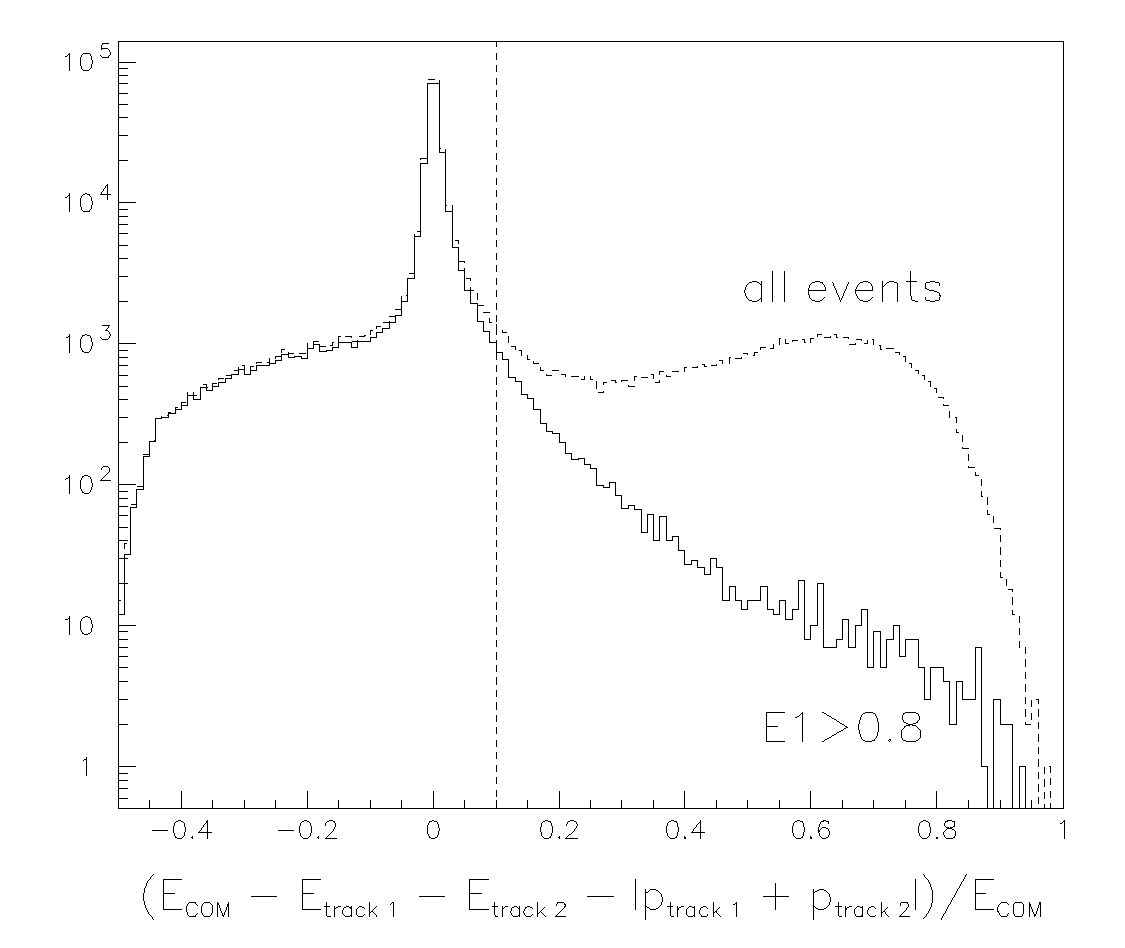
\includegraphics[width=\linewidth]{bhabha_discrimination.pdf}
    \end{minipage} & 
    \begin{minipage}{\linewidth}
      \hypertarget{lastplot}{\mbox{ }} \href{#cutseffective}{[Back]}
    \end{minipage}
  \end{tabular}
\end{lastslide}

\end{document}



%% 1. - CDF[ChiSquareDistribution[9-1], 12.6516285349] (* new hadron, new gamgam *)

%% Out[4]= 0.124411

%% 1. - CDF[ChiSquareDistribution[9-1], 20.9166693414] (* old hadron, new gamgam *)

%% Out[5]= 0.00737211

%% 1. - CDF[ChiSquareDistribution[9-1], 25.7198624176] (* old hadron, old gamgam *)

%% Out[6]= 0.0011727
